\documentclass{article}
\usepackage{graphicx} % Required for inserting images

\usepackage{amsmath}


\usepackage{tikz}
\usepackage{tikz-network}
\usetikzlibrary{positioning}

\tikzset{%
   neuron missing/.style={
    draw=none,
    scale=2,
    text height=0.333cm,
    execute at begin node=\color{black}$\vdots$
  },
}

% The command \DrawNeuronalNetwork has a list as argument, each entry is a layer.
% Each entry has the form:
% Layer name/number of nodes/color/missing node (dots)/label/symbolic number
%
% * "layer name" is the name of the layer
% * "number of nodes" is the number of neurons in that layer (including the missing neuron)
% * "color" is the color of the layer
% * "missing node" denotes the index of the missing neuron, replaced by the dots
% * "label" denotes the label of the layer
% * "symbolic number" denotes the symbol that indicates how many neurons there are

\newcommand{\DrawNeuronalNetwork}[2][]{
\xdef\Xmax{0}
\foreach \Layer/\X/\Col/\Miss/\Lab/\Count [count=\Y] in {#2}
{\pgfmathsetmacro{\Xmax}{max(\X,\Xmax)}
 \xdef\Xmax{\Xmax}
 \xdef\Ymax{\Y}
}
\foreach \Layer/\X/\Col/\Miss/\Lab/\Count [count=\Y] in {#2}
{\node[anchor=south] at ({2*\Y},{\Xmax/2+0.1}) {\Layer};
 \foreach \m in {1,...,\X}
 {
  \ifnum\m=\Miss
   \node [neuron missing] (neuron-\Y-\m) at ({2*\Y},{\X/2-\m}) {};
  \else
   \node [circle,fill=\Col!50,minimum size=1cm] (neuron-\Y-\m) at
  ({2*\Y},{\X/2-\m}) {};
 \ifnum\Y=1
  \else
   \pgfmathtruncatemacro{\LastY}{\Y-1}
   \foreach \Z in {1,...,\LastX}
   {
    \ifnum\Z=\LastMiss
    \else
     \draw[->] (neuron-\LastY-\Z) -- (neuron-\Y-\m);
    \fi
    }
  \fi
 \fi
 \ifnum\Y=1
  \ifnum\m=\X
   \draw [<-] (neuron-\Y-\m) -- ++(-1,0) node [above, midway] {$\Lab_{\Count}$};
  \else
   \ifnum\m=\Miss
   \else
    \draw [<-] (neuron-\Y-\m) -- ++(-1,0) node [above, midway] {$\Lab_{\m}$};
   \fi
  \fi
 \else
   \ifnum\Y=\Ymax
    \ifnum\m=\X
     \draw [->] (neuron-\Y-\m) -- ++(1,0) node [above, midway] {$\Lab_{\Count}$};
    \else
     \ifnum\m=\Miss
     \else
      \draw [->] (neuron-\Y-\m) -- ++(1,0) node [above, midway] {$\Lab_{\m}$};
     \fi
    \fi
   \else
     \ifnum\m=1
      \node[above=0pt of neuron-\Y-\m] {$\Lab_1$};
     \fi
     \ifnum\m=\X
      \node[below=0pt of neuron-\Y-\m] {$\Lab_{\Count}$};
     \fi
   \fi
 \fi
 }
 \xdef\LastMiss{\Miss}
 \xdef\LastX{\X}
}
}
\usepackage{color}

\definecolor{chapter1_orange}{RGB}{253, 192, 134} % rgb(253,192,134)
\definecolor{chapter1_light_orange}{RGB}{253, 192, 134} % rgb(253,192,134)

\definecolor{chapter1_blue}{RGB}{37, 150, 190} % rgb(37, 150, 190)
\definecolor{chapter1_light_blue}{RGB}{146, 203, 223} % rgb(146, 203, 223)

\definecolor{chapter1_green}{RGB}{159, 188, 43} % rgb(159,188,43)
\definecolor{chapter1_light_green}{RGB}{207, 221, 149} % rgb(207,221,149)

\definecolor{chapter1_yellow}{RGB}{255, 205, 64} % rgb(255, 205, 64)
\definecolor{chapter1_light_yellow}{RGB}{255, 230, 59} % rgb(255, 230, 159)

\definecolor{chapter1_red}{RGB}{252, 76, 70} % rgb(252,76,70)
\definecolor{chapter1_light_red}{RGB}{250, 155, 153} % rgb(250,155,153)

% chapter 3

\definecolor{chapter3_red}{RGB}{250,155,153} % rgb(250,155,153)

\definecolor{chapter3_orange}{RGB}{247,187,150} % rgb(247,187,150)

\definecolor{chapter3_yellow}{RGB}{246,210,152} % rgb(246,210,152)

\definecolor{chapter3_blue}{RGB}{115,190,222} % rgb(115,190,222)

\title{Neural Networks}
\author{Daniel Gigliotti}
\date{}

\begin{document}

\maketitle

\section{Shallow Neural Networks}

\vspace{0.5cm}
\begin{center}
    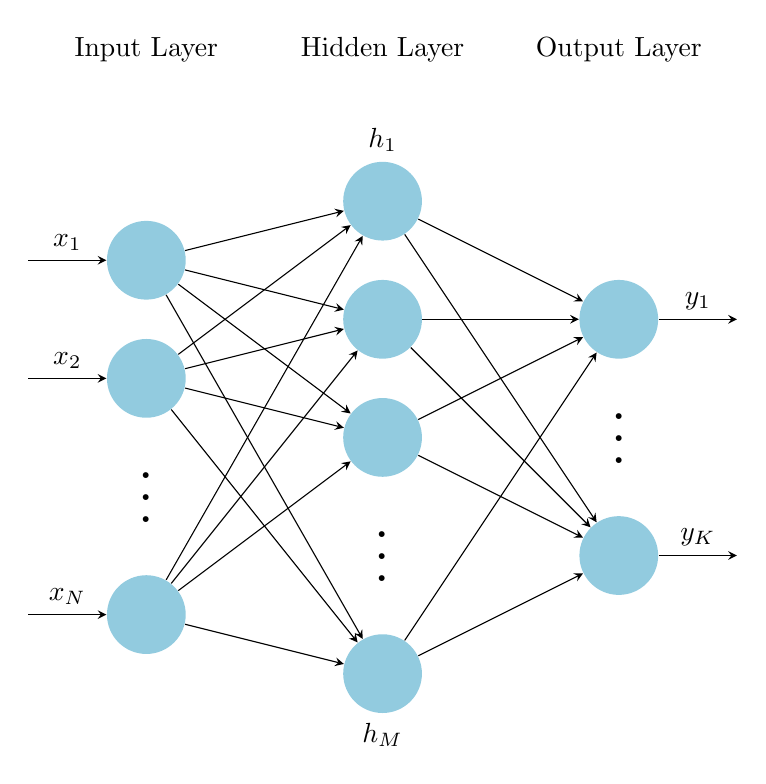
\begin{tikzpicture}[x=1.5cm, y=1.5cm, >=stealth]
        \DrawNeuronalNetwork{
            Input Layer/4/chapter1_blue/3/x/N,
            Hidden Layer/5/chapter1_blue/4/h/M,
            Output Layer/3/chapter1_blue/2/y/K
        }
    \end{tikzpicture}
\end{center}
\vspace{0.5cm}

We would want to describe the general equation for a shallow neural network $y = f[x, \theta]$ that maps a multi-dimensional input $x \in R^N$ to a multi-dimensional output $y \in R^K$ using $h \in R^M$ hidden units. Each hidden unit is computed as:

\begin{equation*}
    h_d = a\big[\theta_{d,0} + \sum_{i=1}^{M_d} \theta_{d,i} x_i \big]
\end{equation*}

These hidden units are combined linearly to create the output:

\begin{equation*}
    y_j = \rho_{j0} + \sum_{d=1}^{D} \rho_{jd} h_d 
\end{equation*}

\textbf{Shallow neural networks} have a relatively small number of hidden layers. \\

The \textbf{total number of parameters} of the network can be found with:

\begin{equation*}
    p = \sum_{l}^{L} (D_i + 1) * D 
\end{equation*}

Where $D$ is the number of units in the current layer and $D_i$ the number of units in input to the current layer. 

For example, for a network with $D_I$ inputs, $D_O$ outputs and $D$ hidden units, the number of parameters is:

\begin{equation*}
    (D_I + 1) * D + (D + 1) * D_O        
\end{equation*}

We will mostly use the ReLU, that has the merit of being easily interpretable. With ReLU activations, the network divides the input space into convex polytopes defined by the intersections of hyperplanes. Assuming we are using the ReLU as activation function, that perfectly splits an hyperplane into two parts on a single joint, the \textbf{maximum number of regions} created by a shallow neural network with $D_I$ inputs, $D_O$ outputs and $D$ hidden units is given by \textbf{Zaslavsky's formula}:

\begin{equation*}
    \sum_{j=0}^{D_i} \binom{D}{j}
\end{equation*}

(that is the maximum number of regions created by partitioning a $D_I$-dimensional space with $D$ hyperplanes). For example, the maximum number of regions created by a shallow network with a $D_I = 2$ dimensional input, $D_O = 1$ dimensional output and $D = 3$ hidden units is:

\begin{equation*}
    N = \binom{3}{0} + \binom{3}{1} + \binom{3}{2} = 1 + 3 + 3 = 7
\end{equation*}

If we increase the number of hidden units to this model so that $D = 5$ we have:

\begin{equation*}
    N = \binom{5}{0} + \binom{5}{1} + \binom{5}{2} = 1 + 5 + 10 = 16
\end{equation*}

\newpage

\section{Deep Neural Networks}

Both deep and shallow networks can model arbitrary functions, but some functions can be approximated much more efficiently with deep networks. It has been found that shallow neural networks need exponentially more neurons to model a function the same way of a deep neural networks i.e. with deep neural networks we have an exponential number of linear regions in the number of hidden layers and this allows us to better approximate any given function. This phenomenon is referred to as the \textbf{depth efficiency of neural networks}.

\end{document}
